

\section{Algorithme Parareal}
\label{sec:algorithme_parareal}

\subsection{Principe fondamental}
L'algorithme Parareal introduit une approche qui brise la barrière de la séquentialité temporelle inhérente aux méthodes classiques. Le principe fondamental repose sur une décomposition du domaine temporel combinée à un processus itératif de correction.

\noindent Cette approche résout les limitations de RK4 en :
\begin{itemize}
    \item Permettant le calcul parallèle sur différents intervalles de temps
    \item Maintenant la précision grâce au propagateur fin
    \item Assurant la convergence via le processus itératif de correction
\end{itemize}

\subsection{Décomposition temporelle}
L'intervalle de temps global est divisé en $N$ sous-intervalles :
\begin{equation}
[0,T] = \bigcup_{i=0}^{N-1} [T_i,T_{i+1}]
\end{equation}

Cette décomposition permet une distribution naturelle du calcul sur plusieurs processeurs, chacun traitant un sous-intervalle spécifique.

\begin{figure}[h]
    \centering
    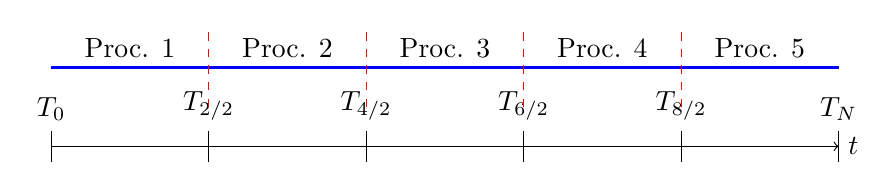
\begin{tikzpicture}[scale=1.0]
        % Axe temporel
        \draw[->] (0,0) -- (10,0) node[right] {$t$};
        \draw (0,-0.2) -- (0,0.2) node[above] {$T_0$};
        \draw (10,-0.2) -- (10,0.2) node[above] {$T_N$};
        
        % Subdivisions
        \foreach \x in {2,4,6,8} {
            \draw (\x,-0.2) -- (\x,0.2) node[above] {$T_{\x/2}$};
        }
        
        % Intervalles parallèles
        \foreach \x in {0,2,4,6,8} {
            \draw[blue, thick] (\x,1) -- (\x+2,1);
            \node[above] at (\x+1,1) {Proc. \number\numexpr\x/2+1};
        }
        
        % Points de synchronisation
        \foreach \x in {2,4,6,8} {
            \draw[red,dashed] (\x,0.5) -- (\x,1.5);
        }
    \end{tikzpicture}
    \caption{Décomposition temporelle et distribution sur les processeurs}
    \label{fig:decomposition}
\end{figure}


\subsection{Architecture à deux niveaux}
L'algorithme repose sur l'utilisation de deux propagateurs complémentaires :

\begin{enumerate}
    \item \textbf{Propagateur grossier $\mathcal{G}$} :
    \begin{itemize}
        \item Rapide mais approximatif
        \item Utilisé pour la prédiction initiale
        \item Typiquement basé sur une méthode d'Euler
    \end{itemize}
    
    \item \textbf{Propagateur fin $\mathcal{F}$} :
    \begin{itemize}
        \item Précis mais coûteux en calcul
        \item Appliqué en parallèle sur les sous-intervalles
        \item Basé sur RK4 dans notre implémentation
    \end{itemize}
\end{enumerate}

\subsection{Processus itératif}
L'algorithme procède en trois phases principales :

\subsubsection{Phase 1 : Initialisation}
\begin{enumerate}
    \item Division de $[0,T]$ en $N$ sous-intervalles
    \item Initialisation : $U_n^0 = u_0$ pour $n = 0$
    \item Prédiction grossière initiale :
    \begin{equation}
        U_{n+1}^0 = \mathcal{G}(T_n, U_n^0, \Delta T) \quad \text{pour } n = 0,\ldots,N-1
    \end{equation}
\end{enumerate}

\subsubsection{Phase 2 : Calcul parallèle}
Pour chaque itération $k$ :
\begin{enumerate}
    \item Calcul en parallèle sur chaque sous-intervalle :
    \begin{equation}
        \mathcal{F}(T_n, U_n^k, \Delta T) \quad \text{pour tout } n
    \end{equation}
    
    \item Application de la formule de correction :
    \begin{equation}
        U_{n+1}^{k+1} = \mathcal{G}(T_n, U_n^{k+1}, \Delta T) + \mathcal{F}(T_n, U_n^k, \Delta T) - \mathcal{G}(T_n, U_n^k, \Delta T)
        \label{eq:correction}
    \end{equation}
\end{enumerate}

\subsubsection{Phase 3 : Test de convergence}
\begin{itemize}
    \item Vérification du critère de convergence :
    \begin{equation}
        \max_n \|U_n^{k+1} - U_n^k\| < \varepsilon
    \end{equation}
    \item Si non convergé et $k < k_{max}$, retour à la Phase 2
\end{itemize}

\subsection{Analyse de la formule de correction}
La formule de correction (\ref{eq:correction}) peut être interprétée comme :
\begin{itemize}
    \item Une prédiction grossière de l'état suivant : $\mathcal{G}(T_n, U_n^{k+1}, \Delta T)$
    \item Une correction basée sur l'erreur du propagateur grossier :
    \begin{equation}
        \delta^k = \mathcal{F}(T_n, U_n^k, \Delta T) - \mathcal{G}(T_n, U_n^k, \Delta T)
    \end{equation}
\end{itemize}

\begin{figure}[h]
    \centering
    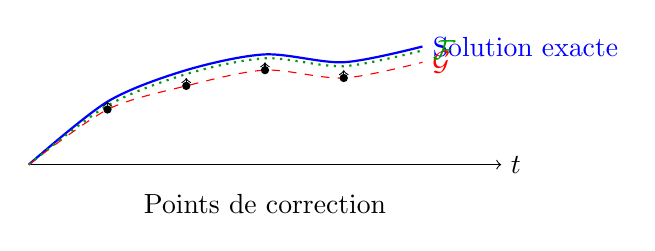
\begin{tikzpicture}[scale=1.0]
        % Axe du temps
        \draw[->] (0,0) -- (6,0) node[right] {$t$};
        
        % Solutions
        \draw[blue, thick] plot[domain=0:5,smooth] coordinates {
            (0,0) (1,0.8) (2,1.2) (3,1.4) (4,1.3) (5,1.5)
        } node[right] {Solution exacte};
        
        \draw[red, dashed] plot[domain=0:5,smooth] coordinates {
            (0,0) (1,0.7) (2,1.0) (3,1.2) (4,1.1) (5,1.3)
        } node[right] {$\mathcal{G}$};
        
        \draw[green!60!black, dotted, thick] plot[domain=0:5,smooth] coordinates {
            (0,0) (1,0.75) (2,1.15) (3,1.35) (4,1.25) (5,1.45)
        } node[right] {$\mathcal{F}$};
        
        % Points de correction
        \foreach \x/\y in {1/0.7, 2/1.0, 3/1.2, 4/1.1} {
            \draw[->] (\x,\y) -- (\x,{\y+0.1});
            \fill (\x,\y) circle (1.5pt);
        }
        
        \node at (3,-0.5) {Points de correction};
    \end{tikzpicture}
    \caption{Illustration du processus de correction}
    \label{fig:correction}
\end{figure}

\subsection{Propriétés de convergence}
La convergence de l'algorithme dépend de plusieurs facteurs :

\begin{enumerate}
    \item \textbf{Qualité du propagateur grossier} :
    \begin{itemize}
        \item Doit capturer suffisamment bien la dynamique du système
        \item Compromis entre précision et rapidité
    \end{itemize}
    
    \item \textbf{Taille des sous-intervalles} :
    \begin{itemize}
        \item Impact sur la vitesse de convergence
        \item Influence sur l'efficacité de la parallélisation
    \end{itemize}
    
    \item \textbf{Nature du système} :
    \begin{itemize}
        \item Sensibilité aux conditions initiales
        \item Non-linéarités et raideur
    \end{itemize}
\end{enumerate}

\subsection{Application au système de Lorenz}
Pour le système de Lorenz modifié étudié, l'application de l'algorithme Parareal nécessite une attention particulière à plusieurs aspects spécifiques :

\subsubsection{Adaptation des propagateurs}
\begin{enumerate}
    \item \textbf{Propagateur grossier $\mathcal{G}$} :
    \begin{itemize}
        \item Utilisation d'une méthode de RK2 :
        \begin{equation}
        \begin{cases}
            X_{n+1} = X_n + \Delta t(Y_n - X_n) \\
            Y_{n+1} = Y_n + \Delta t(-\frac{1}{\tau}Y_n + X_nZ_n) \\
            Z_{n+1} = Z_n + \Delta t(R - \frac{1}{\tau}Z_n - X_nY_n)
        \end{cases}
        \end{equation}
        \item Pas de temps adaptatif basé sur $\tau$ :
        \begin{equation}
        \Delta t_{\mathcal{G}} = \min(\alpha\tau, \Delta T)
        \end{equation}
        où $\alpha$ est un facteur de sécurité ($\approx 0.1$)
    \end{itemize}

    \item \textbf{Propagateur fin $\mathcal{F}$} :
    \begin{itemize}
        \item Méthode RK4 avec pas de temps fin :
        \begin{equation}
        \Delta t_{\mathcal{F}} = \frac{\Delta t_{\mathcal{G}}}{m}
        \end{equation}
        où $m$ est typiquement choisi entre 10 et 100
        \item Conservation des invariants du système
    \end{itemize}
\end{enumerate}

\subsubsection{Considérations dynamiques}
Les caractéristiques particulières du système influencent l'application de Parareal :

\begin{enumerate}
    \item \textbf{Régimes de comportement} :
    \begin{itemize}
        \item Régime transitoire : nécessite une plus grande précision du propagateur grossier
        \item Régime établi : permet des pas de temps plus grands
        \item Zones de bifurcation : requiert une attention particulière
    \end{itemize}

    \item \textbf{Échelles de temps} :
    \begin{figure}[h]
        \centering
        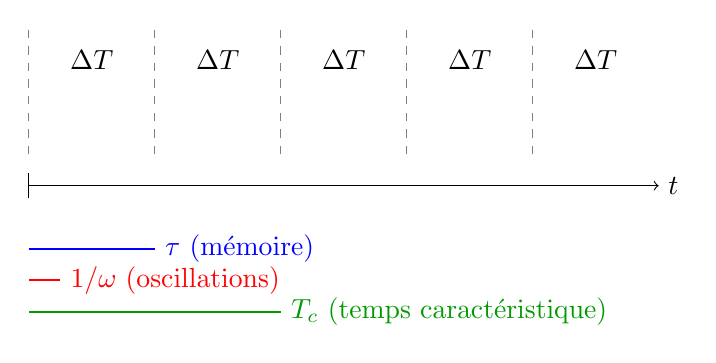
\begin{tikzpicture}[scale=0.8]
            % Axe temporel avec échelles
            \draw[->] (0,0) -- (10,0) node[right] {$t$};
            \draw (0,-0.2) -- (0,0.2);
            
            % Échelles caractéristiques
            \draw[blue,thick] (0,-1) -- (2,-1) node[right] {$\tau$ (mémoire)};
            \draw[red,thick] (0,-1.5) -- (0.5,-1.5) node[right] {$1/\omega$ (oscillations)};
            \draw[green!60!black,thick] (0,-2) -- (4,-2) node[right] {$T_c$ (temps caractéristique)};
            
            % Décomposition Parareal
            \foreach \x in {0,2,4,6,8} {
                \draw[gray,dashed] (\x,0.5) -- (\x,2.5);
                \node at (\x+1,2) {$\Delta T$};
            }
        \end{tikzpicture}
        \caption{Différentes échelles de temps du système}
        \label{fig:echelles_temps}
    \end{figure}
    
    \item \textbf{Impact du paramètre $\tau$} :
    \begin{itemize}
        \item Influence sur la taille optimale des sous-intervalles
        \item Ajustement de la fréquence des points de synchronisation
        \item Configuration du ratio $\Delta t_{\mathcal{F}}/\Delta t_{\mathcal{G}}$
    \end{itemize}
\end{enumerate}

\subsubsection{Stratégies de convergence}
Pour assurer une convergence efficace, plusieurs stratégies sont mises en place :

\begin{enumerate}
    \item \textbf{Critères adaptatifs} :
    \begin{equation}
    \varepsilon_k = \max\left\{\frac{\|U_n^{k+1} - U_n^k\|}{\|U_n^k\|}, \frac{|E_k - E_{k-1}|}{|E_k|}\right\} < \text{tol}
    \end{equation}
    où $E_k$ est l'énergie du système à l'itération $k$

    \item \textbf{Décomposition intelligente} :
    \begin{itemize}
        \item Intervalles plus courts dans les zones de forte non-linéarité
        \item Adaptation basée sur les estimateurs d'erreur locale
        \item Équilibrage de charge entre processeurs
    \end{itemize}

    \item \textbf{Gestion des instabilités} :
    \begin{itemize}
        \item Détection précoce des divergences
        \item Mécanismes de repli sur des pas plus petits
        \item Conservation des quantités physiques importantes
    \end{itemize}
\end{enumerate}

\subsubsection{Optimisations spécifiques}
Plusieurs optimisations sont implémentées pour améliorer l'efficacité :

\begin{itemize}
    \item \textbf{Prédiction améliorée} :
    \begin{equation}
    U_{n+1}^0 = \mathcal{G}(T_n, U_n^0, \Delta T) + \beta(U_n^0 - U_{n-1}^0)
    \end{equation}
    où $\beta$ est un facteur d'extrapolation basé sur la dynamique locale

    \item \textbf{Réutilisation des calculs} :
    \begin{itemize}
        \item Stockage intelligent des états intermédiaires
        \item Mise en cache des trajectoires partielles
        \item Réduction des communications MPI
    \end{itemize}

    \item \textbf{Adaptation dynamique} :
    \begin{itemize}
        \item Ajustement automatique des paramètres
        \item Modification de la décomposition en cours d'exécution
        \item Équilibrage de charge basé sur les performances observées
    \end{itemize}
\end{itemize}

Ces considérations spécifiques au système de Lorenz permettent d'optimiser l'efficacité de l'algorithme Parareal tout en maintenant la précision nécessaire pour capturer correctement la dynamique du système.